%enunciado
Muchos estudios buscan relacionar variables del entorno con enfermedades y as\'i dar con las causas de
\'estas y as\'i poder tomar un plan de acci\'on adecuado. En el siguiente caso, se tomaron muestras de agua
y se midi\'o su grado de contaminaci\'on. Adem\'as se guarda un registro del promedio de personas enfermas
que pertenecen al \'Area de donde se han tomado las muestras de agua. Los datos son los siguientes:\\
\begin{tabular}{|l|c|c|c|c|c|c|c|c|c|c|c|c|r|}
	\hline
     Zona                   & A & B   & C  & D   & E    & F  & G   & H   & I   & J    & K  & M \\  \hline
     Nivel de Contaminacion & 1 & 8   & 3  & 15  & 18   & 5  & 9   & 14  & 2   & 21   & 4  & 18 \\  \hline
     Promedio enfermos      & 2 & 185 & 20 & 835 & 1378 & 63 & 240 & 699 & 425 & 1983 & 37 & 1539 \\ \hline
\end{tabular}\\
\begin{itemize}
	\item Proponga un modelo de regresi\'on lineal que explique la incidencia de la enfermedad en
	 t\'erminos de la contaminaci\'on del agua. Si es necesario, aplique una transformaci\'on a los
	 datos.
	%respuesta
	\begin{center}
		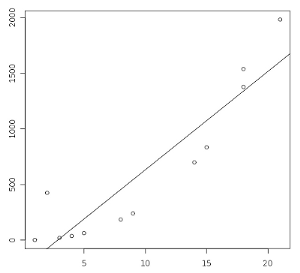
\includegraphics[height=6cm]{images/preg3}
	\end{center}
	concluir acerca de como se relacionan, sin olvidar que posee una forma exponencial.\\
	aplicar transformacion exponencial
  	\item Evalue si el modelo obtenido modela de manera razonable los datos.
	%respuesta
	una vez hecha la transformacion se dice que se modela bien los datos por bla bla bla
	\item ?`Aprecia alg\'un dato at\'ipico que podr\'ia influenciar la conclusi\'on anterior? Explique.
	%respuesta
	hay que ver losd atos que estan sobrando para que la transformacion exponencial no se netamente
	exponencial, por ejemplo, (8,185),(18,1539), basta ver el dibujo 
	\item Si el muestreo de las aguas se hizo por conveniencia, ?`qu\'e validez tienen las
	conclusiones obtenidas?
	%respuesta
	En el Muestreo por conveniencia, los elementos de la muestra se eligen por estar en el  lugar o en
	el momento adecuado para la investigacio\'on, por lo tanto este estudio pierde un poco de validez
	ya que no representa una muestra de agua de cualquier casa por ejemplo. sino que se espero el momento
	preciso donde se toparon con agua contaminada, para poder realizarlo.

\end{itemize}
